%!TEX root = ../PTC-LibUG.tex
\makeusother
\linenumberfrequency{5}

\chapter{Modeling an Accelerator with \PTC}
\label{cha:model.accel}

\fxnote{Review underscore (\_\,) characters in index entries.}
\fxnote{Review percent (\%\,) characters in index entries.}
\fxnote{Review line numbers.}

\index{accelerator!modeling tutorial}
\index{modeling!accelerator topologies}
%
This chapter explains how to use \PTC\ to model the geometry for a
range of accelerators. To that end, we introduce three accelerator
topologies and show how to define their geometries using \PTC. After
going through these models in detail, you should have a good
understanding of how to use \PTC\ to model your own accelerator
designs. If some of your elements move together as units---because
they're tied to a girder, for example---then you will also want to
absorb the information presented in \CTref*{girders}.

In \Sref{accel.models} we describe briefly the accelerator topologies
we shall model. In \Sref{geom.tut} we introduce the \PTC\ source code
for our examples. The three accelerator topologies use some common
structures, and we describe the subroutines for these in
\Sref{geom.sub}. Then, in \Sref[s]{pop.DNA} and \Sref*{model.topos},
we construct our \DNA\ sequences and show in detail how to construct
our three accelerator designs. We conclude, in \Sref{DNA.array}, with
some housekeeping
\fxnote{Is there a better word than ``housekeeping''?}
for our \DNA\ database.

%The goal of this chapter is to explain how to model the geometry
%of an accelerator in \PTC. This chapter introduces three accelerator
%topologies, and explains how to define the geometry of those models
%in a \PTC\ source file.

%\PTC, as mentioned earlier in the \Tref{cha:overview}, separates
%the geometry of accelerators from their properties, such as particle
%trajectories. For that reason, this chapter does not discuss the
%computation of accelerator properties. For information about how to
%use Taylor maps derived from the integrator to compute lattice
%functions, see \TCref*{polymorphs.knobs}.


\section{Accelerator Models}
\label{sec:accel.models}

\index{accelerator topology!model of ring with forward and reverse propagation}
\index{accelerator topology!model of figure eight}
\index{accelerator topology!model of collider}
\index{ring with forward and reverse propagation!modeling}
\index{figure-eight accelerator!modeling}
\index{collider!modeling}
%
\fref[c]{accel.models} illustrates the three accelerator topologies
we shall model:
\begin{itemize}
  \item figure-eight,
  \item ring with both forward and reverse propagation,
  \item collider.
\end{itemize}
All three machines are based on a ten-cell ring, with each cell
composed of seven elements: a drift, a focusing quadrupole, a short
drift, a dipole, a short drift, a defocusing quadrupole, and another
drift.%
\sidenote{When you see the particular numbers, in a few pages, you
may recognize this cell as that of the Los Alamos Proton Storage Ring.}
In the figure-eight and collider examples, the dipole is a rectangular
bend. In the ring with forward and reverse propagation, however, the
dipole is what we shall call, for want of a better term, a
\emph{``straight'' bend} (with the quotation marks!). By this we shall
mean a rectangular bending magnet whose entrance and exit reference
frames are parallel to one another and orthogonal to the main axis of
the magnet. This implies---see \TPref*{sec:chart.patch}---that any cell
containing a ``straight'' bend will require patching.

\begin{figure}[htb]\forceversofloat
  \centering
  %\includegraphics[width=\linewidth]{illustrations/model-cell}\\
  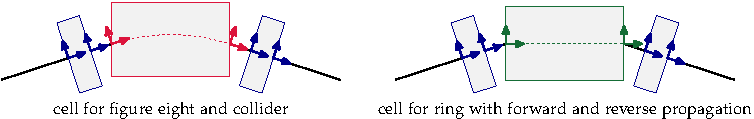
\includegraphics{Layouts/models-00}
  \caption{Basic cells for the three accelerator models.}
  \label{fig:basic.cells}
\end{figure}

\fref[c]{basic.cells} illustrates the two basic cells. We outline
the quadrupoles in blue, the rectangular bend in red, and the
``straight'' bend in green. The black lines indicate the drifts.
The cell with the rectangular bend does not require patching (unless
the direction or charge change), because the reference frames of
adjacent elements lie on top of one another. The cell with the
``straight'' bend, however, requires patching (regardless of
direction or charge), because the adjacent drifts have frames that
are rotated with repect to those of the ``straight'' bend.

\index{build\_PSR@\ptc{build\_PSR}!basic ring}
%
The basic ring (see the \ptc{build_PSR} example in \fref{DNA.subrtns}
on \pref{fig:DNA.subrtns}) has ten cells. It has 70~fibres, each pointing
to one of 70~elements. The ring with forward and reverse propagation has
140~fibres pointing to 140~elements.

The figure-eight and the collider each have 140~fibres pointing to
134~elements. In each of those models the upper and lower rings share
the elements at the start of one cell (long drift, quadrupole, short
drift) and the elements at the end of another cell (short drift,
quadrupole, long drift).

\begin{figure}[ht]
  \centering
  %\includegraphics[width=\textwidth]{illustrations/model-tutorial}
  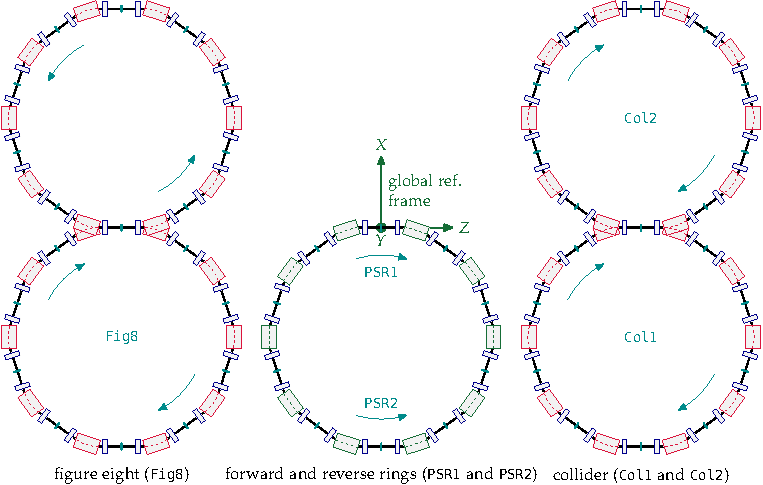
\includegraphics{Layouts/models-01}
  \caption{Accelerator models. Arrows indicate the direction of motion
           of particle beams in the constituent layouts.}
  \label{fig:accel.models}
\end{figure}

Our three tutorial examples are not real accelerators: They do not
have particle injectors or dumps; and two of the examples are not
physically possible, because some of their elements overlap in space.
The goal of these examples is to introduce the principal \PTC\ concepts
involved in modeling the geometry of an accelerator. After learning
these concepts, we can use \PTC\ to model complex real-world
accelerators.


\section{Geometry Tutorial Source File}
\label{sec:geom.tut}

\index{PTC!source file}
\index{source file!geometry tutorial}
\index{geometry!tutorial source file}
\index{ptc\_geometry.f90@\ptc{ptc\_geometry.f90}!geometry tutorial source file}
%
The example code in this chapter is from the \PTC\ geometry tutorial
source file, \ptc{ptc_geometry.f90}, which is given in
\Aref{geom.tutorial}. The line numbers of the code in the examples
refer to the line numbers of the code in that appendix.


\subsection{Initial Code}
\label{sec:init.code}

The initial code in the \ptc{ptc_geometry.f90} source file
includes type declarations and performs some initialization.

\setptclinenums{1}{5}
\begin{ptccode}[
  label={\ptctitle{\ptc{ptc_geometry.f90}\quad\small This program
                   describes the geometry of several \PTC\ lattices.}}
]
program ptc_geometry
use run_madx
use pointer_lattice
implicit none

character*48 :: command_gino    \label{lin:gino}
logical(lp) :: doit
integer :: i, j, mf, pos, example
real(dp) :: b0
real(dp), dimension(3) :: a, d  \label{lin:decl.ad}
real(dp), dimension(6) :: fix1, fix2, mis, x
type(real_8), dimension(6) :: y1, y2
type(layout), pointer :: L1, L2, L3, L4, L5, L6
type(layout), pointer :: PSR1, PSR2, Fig8, Col1, Col2
type(fibre), pointer :: p1, p2, p3, pf, b, f
type(internal_state) :: state

type(pol_block) :: qf(2), qd(2)
type(normalform) :: n1, n2
type(damap) :: id
type(taylor) :: eq(4)
type(gmap) :: g
!-----------------------------------

Lmax = 100.d0
use_info = .true.

! one layout necessary before starting GUI
call ptc_ini_no_append          \label{lin:init.layout}
\end{ptccode}

\fxnote{What does \ptc{use\_info = .true.} do?!?}

\index{PTC!universe}
\index{universe!PTC}
\index{MAD universe|see{PTC universe}}
\index{global variable!\ptc{m\_u}}
\index{m\_u@\ptc{m\_u}!global variable}
\index{DNA database!\ptc{m\_u} global variable}
\index{module!\ptc{madx\_ptc\_module}}
\index{madx\_ptc\_module@\ptc{madx\_ptc\_module}!module}
\index{linked list!\ptc{m\_u} global variable}
%
The module \ptc{run_madx} tells \PTC\ to use the
\ptc{madx_ptc_module}, which defines the global variable
\ptc{m_u}.\label{mad.univ}%
\sidenote{Think "\emph{M}\textsc{ad} \emph{U}niverse".}
This variable, which we shall use frequently, denotes a linked list
of layouts%
\sidenote{We use the linked-list aspect of \ptc{m_u} only briefly
in \STref{DNA.array}.}
that will constitute our \DNA\ database. The \ptc{gino}
mentioned on \lref{gino} refers to a
Windows$^\text{\textregistered}$-based graphical user
interface developed for \PTC\ by \'Etienne Forest.
Its use is not required.

\PTC\ uses the following type declarations for modeling accelerator
topologies:
\begin{itemize}
  \item \ptc{real(dp)} for double precision real numbers,
  \item \ptc{type(layout)} for \ptctyp{layout}s,
  \item \ptc{type(fibre)} for \ptctyp{fibre}s,
  \item \ptc{type(internal_state)} for setting the characteristic
         dynamics desired of your accelerator (see \TAref*{states}).
\end{itemize}
These data types will be discussed in this chapter.

\PTC\ uses the following type declarations for analyzing accelerator
properties:
\begin{itemize}
  \item \ptc{type(real_8)} for polymorphs,
  \item \ptc{type(pol_block)} for polymorphic blocks,
  \item \ptc{type(normalform)} for normal forms,
  \item \ptc{type(damap)} for a vector of Taylor maps
        (differential algebra maps),
  \item \ptc{type(taylor)} for single Taylor maps,
  \item \ptc{type(gmap)} for a vector of Taylor maps.
\end{itemize}
These latter data types will be described in \CTref*{polymorphs.knobs}.

\index{global variable!\ptc{lmax}}
\index{lmax@\ptc{lmax}!global variable}
\index{integration node!setting maximum length}
%
The global variable \ptc{Lmax} defines the maximum length (here
100~meters!) of an integration node. For more information about
splitting elements into integration nodes,
see \TCref*{symplectic.integ}.

This initial code also, on \lref{init.layout}, initializes a layout;
this must be done before starting \PTC's
Gino$^\text{\textregistered}$-based graphical user interface for Windows.


\section{Subroutines}
\label{sec:geom.sub}

\index{DNA sequence!example source code}
\index{DNA database!example source code}
%
The end of the \ptc{ptc\_geometry.f90} source file contains three
subroutines we use to create the \DNA\ sequences---non-trackable
layouts for our \DNA\ database. \fref[c]{DNA.subrtns} shows the
layouts that the three subroutines create. In subsequent sections
of this chapter, we describe how to use the layouts from this database,
or pieces of these layouts, to form the accelerator models of
\fref{accel.models}.

\begin{figure}[ht]
  \centering
  %\includegraphics[width=\linewidth]{illustrations/model-PSR}
  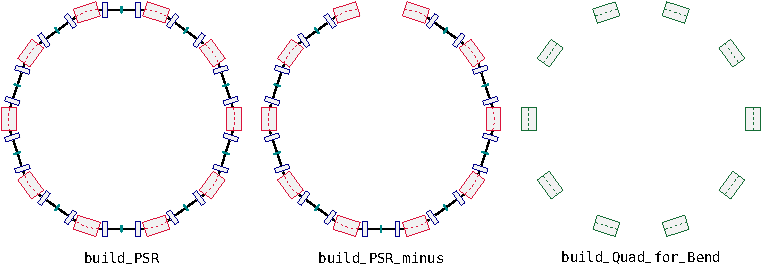
\includegraphics{Layouts/models-02}
  \caption{Subroutines for creating \DNA\ sequences.}
  \label{fig:DNA.subrtns}
\end{figure}


\subsection{build\_PSR}
\label{sec:build.psr}

\index{build\_PSR@\ptc{build\_PSR}!example source code}
%
The subroutine \ptc{build_PSR} creates the basic ten-cell ring
lattice shown on the left in \fref{DNA.subrtns}.

\setptclinenums{490}{5}
\begin{ptccode}
subroutine  build_PSR(PSR)
use run_madx
use pointer_lattice
implicit none

type(layout), target :: PSR

real(dp) :: ang, brho, kd, kf, Larc
type(fibre) :: b, d1, d2, qd, qf
type(layout) :: cell
!-----------------------------------

call make_states(.false.)       \label{lin:bptc.psrstates}
exact_model = .true.
default = default + nocavity + exactmis
call update_states
madlength = .false.             \label{lin:eptc.psrstates}

ang = (twopi * 36.d0 / 360.d0)
Larc = 2.54948d0
brho = 1.2d0 * (Larc / ang)
call set_mad(brho = brho, method = 2, step = 10) \label{lin:psr.setmad}
madkind2 = drift_kick_drift

kf =  2.72d0 / brho
kd = -1.92d0 / brho

d1 = drift("D1", 2.28646d0)     \label{lin:bptc.psrlatt}
d2 = drift("D2", 0.45d0)
qf = quadrupole("QF", 0.5d0, kf)
qd = quadrupole("QD", 0.5d0, kd)
b  = rbend("B", Larc, ang) \label{lin:psr.bend}
cell = d1 + qd + d2 + b + d2 + qf + d1 \label{lin:eptc.psrlatt}

PSR = 10 * cell
PSR = .ring.PSR                 \label{lin:psr.ring}

call survey(PSR)
end subroutine build_PSR
\end{ptccode}

\index{internal states!example source code}
\index{state!internal}
\index{make\_states@\ptc{make\_states}!routine}
\index{routine!\ptc{make\_states}}
\index{exact\_model@\ptc{exact\_model}!global parameter}
\index{global parameter!\ptc{exact\_model}}
\index{madlength@\ptc{madlength}!flag}
\index{flag!\ptc{madlength}}
%
\glossary[ptccmds](make\_states)%
  {make\_states(<\textit{\normalfont{bool}}>)}%
  {This subtoutine sets internal-state variables associated
   with the particle type.
   In particular, use \ptc{call make\_states(true)} for electrons,
   and \ptc{call make\_states(false)} for protons.}
%
The \lref[s]{bptc.psrstates}--\lref*{eptc.psrstates} set important
internal state variables for tracking. In the call to
\ptc{make_states}, the boolean argument \ptc{.false.} means we are
modeling a proton lattice. Use \ptc{.true.} for electrons.%
\sidenote{For other particles, use the ratio of particle mass to
electron mass as the argument of \ptc{make_states}.}
To use the full ``square-root'' Hamiltonian, we set the global
parameter \ptc{exact_model} to \ptc{.true.} The global variable
\ptc{default}, of type \ptctyp{internal_state}, is here modified
from its default value by adding the following two flags:
\begin{itemize}
  \item \ptc{nocavity}, which tells \PTC\ to ignore RF cavities;
  \item \ptc{exactmis}, which tells \PTC\ to treat misalignments exactly.
\end{itemize}
(For more on internal-state variables, see \Aref{states}.)
Finally, we set the flag \ptc{madlength} to \ptc{.false.} This
means that \PTC\ will use the arc length, rather than the chord
length, to define the geometry of a rectangular bending magnet.
Use \ptc{.true.} to make \PTC\ use the chord length.

\begin{marginfigure}\forcerectofloat
  %\includegraphics{illustrations/rbend}
  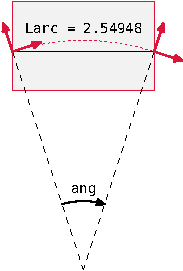
\includegraphics{Layouts/models-04}
  \caption{Geometry of the rectangular bend.}
  \label{fig:rect.bend}
\end{marginfigure}

\fxnote{Need to say something about \ptc{madkind2}.}

\index{set\_mad@\ptc{set\_mad}!routine}
\index{routine!\ptc{set\_mad}}
\index{integration nodes!specifying number of}
\index{energy!specifying}
%
\makeussubscript
\label{set.mad}
The call, in \lref{psr.setmad}, to \ptc{set\_mad} defines (via
\ptc{brho}) the scale momentum $p_o$ for the fibres in the
layout returned by this subroutine. It also specifies the type
(\ptc{method = 2}) and number (\ptc{STEP = 10}) of integration steps
in the body of each element. We then define the five fibres needed
for our basic cell:
\makeusother
\begin{itemize}
  \item Fibres \ptc{d1} and \ptc{d2} denote the long and short drifts.
  \item Fibres \ptc{qf} and \ptc{qd} denote the focusing and defocusing
        quadrupoles.
  \item And fibre \ptc{b} denotes the rectangular bending magnet.
        Note that it is defined by its arc length and bend angle---here
        \ptc{Larc} and \ptc{ang}, respectively.
        See \fref{rect.bend}.
\end{itemize}
The symbols in quotes (\eg, \ptc{"QF"}) are the \emph{names} given
to these elements.%
\sidenote{Because a layout may have any number of these elements,
the names actually define \emph{classes} of elements.}
We may now define the variable \ptc{cell}, of type \ptctyp{layout}, as
the appropriate sequence of fibres. Finally, the layout \ptc{PSR}
returned by this subroutine is defined as 10 cells, and
\lref{psr.ring} modifies \ptc{PSR} to make it a ring, \ie, closed.

\index{survey@\ptc{survey}!routine}
\index{routine!\ptc{survey}}
%
At this point, \lref{psr.ring}, the elements of the \PSR\ lattice
are present, and in the correct sequence of fibres, in layout
\ptc{PSR}. But should we ask for the location of those elements,%
\sidenote{The way to ask this of \PTC\ will become clear later in
this chapter. See, for example, \pref{move.elem}---especially the
discussion of moving and rotating elements.}
we would discover that all of them have their entrance frames at
the global origin.  In other words, they are all stacked on top
of one another at the global origin.
%\linenumberfrequency{0}
%\begin{ptccode}[frame=none]
%  p => PSR%start
%  do i = 1, PSR%n
%    write(mf,'(a)') p%mag%name
%    write(mf,'(a,3(1x,f13.7))') "a:   ", p%chart%f%a
%  end do
%\end{ptccode}
The call to \ptc{survey} causes \PTC\ to loop through the fibres in
\ptc{PSR}, moving each element so that its entrance frame coincides
with the exit frame of the previous element. For the \PSR\ lattice,
the reference frames for the bends and quadrupoles line up exactly
with those of their adjacent drifts. As a consequence, this lattice
requires no patching. We have therefore finished building the
\PSR\ lattice in \PTC.

\newthought{Some readers will complain} that the set of
\lref[s]{bptc.psrlatt} through \lref*{eptc.psrlatt} violates the
philosophy of \PTC---and they have a point. This may seem subtle,
but we urge all other readers to invest the time required to
comprehend this point. Look, for example, at the definition of the
bend given in \lref{psr.bend}. After careful consideration of this
definition and what happens on the succeeding lines, the reader
should recognize that this definition actually serves a dual purpose.
On the one hand, the setting of arc length and bend angle define the
\emph{geometry} of the element. On the other hand, this line also
serves to define the \emph{physics} of this element. To verify this
claim, query \PTC\ for the magnetic field of this element:
\linenumberfrequency{0}
\begin{ptccode}[frame=none]
  write(6,'(a,f7.4)') "PSR B-field = ", b%mag%bn(1) * brho
\end{ptccode}
\linenumberfrequency{5}
will do the trick. You will learn that \PTC\ already knows the
magnetic field has a value of \SI{1.2}{T}! This information, of
course, requires a knowledge of not only the geometry, but also the
particle mass and energy. \emph{Here} is the apparent violation of
the \PTC\ philospophy, which aims to separate the geometric
description of beamline elements (location, reference frames, \etc)
from their physical content (magnetic field strength, \etc). The
resolution of this conflict lies in the fact that once we have
nailed down the geometry, we are then free to modify the lattice
with misalignments, changes to the magnetic field, and the like.


\subsection{build\_PSR\_minus}

\index{build\_PSR\_minus@\ptc{build\_PSR\_minus}!example source code}
%
The subroutine \ptc{build_PSR_minus} defines the partial ring shown
in the center of \fref{DNA.subrtns}. It begins with a bend, a short
drift, a quadrupole, and a long drift; it continues with eight
\PSR\ cells; and it concludes with a long drift, a quadrupole, a short
drift, and a bend. Relative to the \PSR\ lattice, this partial ring is
missing a short drift, a quadrupole, two long drifts, a quadrupole,
and a short drift. The subroutine is a straightforward modification of
that for \ptc{build_PSR}.
%
\fxnote{Actually, this code sets \ptc{method=6} in the call to
\ptc{set\_mad}. Should we change this, or comment on it?}

\linenumberfrequency{5}
\setptclinenums{532}{5}
\begin{ptccode}
subroutine  build_PSR_minus(PSR)
use run_madx
use pointer_lattice
implicit none

type(layout), target :: PSR

real(dp) :: ang, brho, kd, kf, Larc
type(fibre) :: b, d1, d2, qd, qf
type(layout) :: cell
!-----------------------------------

call make_states(.false.)
exact_model = .true.
default = default + nocavity + exactmis
call update_states
madlength = .false.

ang = (twopi * 36.d0 / 360.d0)
Larc = 2.54948d0
brho = 1.2d0 * (Larc / ang)
call set_mad(brho = brho, method = 6, step = 10)
madkind2 = drift_kick_drift

kf =  2.72d0 / brho
kd = -1.92d0 / brho

d1 = drift("D1", 2.28646d0)
d2 = drift("D2", 0.45d0)
qf = quadrupole("QF", 0.5d0, kf)
qd = quadrupole("QD", 0.5d0, kd)
b  = rbend("B", Larc, ang)
cell = d1 + qd + d2 + b + d2 + qf + d1

PSR = b + d2 + qf + d1 + 8 * cell + d1 + qd + d2 + b
PSR = .ring.PSR

call survey(PSR)
end subroutine build_PSR_minus
\end{ptccode}


\subsection{build\_Quad\_for\_Bend}

\index{build\_Quad\_for\_Bend@\ptc{build\_Quad\_for\_Bend}!example source code}
%
The subroutine \ptc{build_Quad_for_Bend} defines the layout shown
on the right in \fref{DNA.subrtns}. It has ten ``straight'' bends,
which have the same length as the rectangular bends in the
\PSR\ lattice. Because the entrance and exit frames of the ``straight''
bends are not rotated, we will need to insert patches everywhere.
These patches will describe both rotations and drifts between the
elements. In fact, because this layout contains no focusing elements,
its entries will be used only in other layouts.

\setptclinenums{574}{5}
\begin{ptccode}
subroutine  build_Quad_for_Bend(PSR)
use run_madx
use pointer_lattice
implicit none

type(layout),target :: PSR

real(dp) :: ang, ang2, brho, b1, Larc, Lq
type(fibre) :: b
!-----------------------------------

call make_states(.false.)
exact_model = .true.
default = default + nocavity + exactmis
call update_states
madlength = .false.

ang = (twopi * 36.d0 / 360.d0)
Larc = 2.54948d0
brho = 1.2d0 * (Larc / ang)
call set_mad(brho = brho, method = 6, step = 10)
madkind2 = drift_kick_drift     \label{lin:qfb.same}

ang2 = ang / two                \label{lin:bptc.qfb.bend}
b1 = ang / Larc
Lq = Larc * sin(ang2) / ang2

b = quadrupole("B_QUAD", Lq, 0.d0);
call add(b, 1, 0, b1)           \label{lin:qfb.b1}
b%mag%permfringe = .true.       \label{lin:bptc.qfb.frng}
b%magp%permfringe = .true.
b%mag%p%bend_fringe = .true.
b%magp%p%bend_fringe = .true.   \label{lin:eptc.qfb.bend}

PSR = 10 * b
PSR = .ring.PSR

call survey(PSR)                \label{lin:qfb.survey}
end subroutine build_Quad_for_Bend
\end{ptccode}

Except for some changes in the type declarations, the code through
\lref{qfb.same} in this subroutine is identical to that in the
previous two subroutines. The ``straight'' bend is created in
\lref[s]{bptc.qfb.bend} through \lref*{eptc.qfb.bend}. We first
compute the length \ptc{Lq} as the chord length of the \PSR's
rectangular bend. To achieve the desired ``straight'' reference
frames, we define the ``straight'' bend as a zero-strength
quadrupole. Then, to make this a dipole, we set, in \lref{qfb.b1},
the normalized dipole strength of \ptc{b} to the computed value
\ptc{b1}. Finally, we set some flags to give this magnet the fringe
fields appropriate to a rectangular bend.

Query: After the call to \ptc{survey} in \lref{qfb.survey}, where
in the global frame are the magnets that this subroutine defines?%
\sidenote{They lie all in a straight line, one after the other,
starting at the global origin and extending to a point 10\,\ptc{Lq}
out along the $z$ axis. Making this layout look like the right-hand
layout of \fref{DNA.subrtns} will require more work.}


\section{Populating the \DNA\ Database}
\label{sec:pop.DNA}

\index{DNA database!populating}
\index{DNA sequence!populating DNA database}
\index{layout!non-trackable}
%
Using the subroutines described in the previous section, we shall
populate our \DNA\ database with six \DNA\ sequences (non-trackable
layouts): \ptc{L1}, \ptc{L2}, \ptc{L3}, \ptc{L4}, \ptc{L5}, and
\ptc{L6}. Note that we shall want each element in our three
accelerator models to appear once and only once in the \DNA-sequence
portion of the \DNA\ database. This uniqueness will reflect the
uniqueness of the individual beamline elements in our accelerators.

\index{layout!trackable}
%
Layouts \ptc{L1} and \ptc{L2} will provide the elements for the
concentric rings accelerator: trackable layouts \ptc{PSR1} and
\ptc{PSR2}. (See \fref{accel.models}.) Layouts \ptc{L3} and \ptc{L4}
will provide the elements for the figure-eight accelerator: trackable
layout \ptc{Fig8}. And layouts \ptc{L5} and \ptc{L6} will provide the
elements for the collider: trackable layouts \ptc{COL1} and \ptc{COL2}.
\tref[c]{DNA.dbase} summarizes the layouts we plan to create: six
\DNA\ sequences, or non-trackable layouts, and the five trackable layouts.

\begin{table}[t]
  \caption{DNA database for the \PTC\ geometry tutorial}
  \label{tbl:DNA.dbase}
  \begin{center}
    \begin{tabular}{ll} \toprule
  Non-trackable layouts & Trackable layouts \\ \midrule
  \ptc{L1}: 70 elements (\ptc{build_PSR}) & 
    \ptc{PSR1}: created from \ptc{L1} and \ptc{L2} \\
  \ptc{L2}: 10 elements (\ptc{build_Quad_for_Bend}) & 
    \ptc{PSR2}: created from \ptc{L1} and \ptc{L2} \\
  \ptc{L3}: 64 elements (\ptc{build_PSR_minus}) & 
    \ptc{Fig8}: created from \ptc{L3} and \ptc{L4} \\
  \ptc{L4}: 70 elements (\ptc{build_PSR}) & 
    \ptc{Col1}: created from \ptc{L6} \\
  \ptc{L5}: 64 elements (\ptc{build_PSR_minus}) & 
    \ptc{Col2}: created from \ptc{L5} and \ptc{L6} \\
  \ptc{L6}: 70 elements (\ptc{build_PSR}) & \\ \bottomrule
    \end{tabular}
  \end{center}
\end{table}

Query: As initially constructed (by \ptc{build_PSR}), layouts \ptc{L1},
\ptc{L4}, and \ptc{L6} are identical. So also are layouts \ptc{L3} and
\ptc{L5}. Why don't we avoid this duplication?%
\sidenote{Because we want to be able to modify---move, mispower,
\etc--- the individual elements. We do not want changes made to
\ptc{COL1}, for example, to appear in \ptc{Fig8}.}

\index{append\_empty\_layout@\ptc{append\_empty\_layout}!routine}
\index{routine!\ptc{append\_empty\_layout}}
\index{global variable!\ptc{m\_u}}
\index{m\_u@\ptc{m\_u}!global variable}
%
The following four lines create the first \DNA\ sequence:
%
\setptclinenums{37}{5}
\begin{ptccode}
call append_empty_layout(m_u) ! DNA sequence 1
call set_up(m_u%end)
L1 => m_u%end
call build_PSR(L1)
\end{ptccode}
%
The call to \ptc{append_empty_layout} appends an empty layout to
the global linked list of layouts \ptc{m_u}. The layout pointer
\ptc{m_u\%end} points to this empty layout. The second line
initializes this new layout; and the third line makes \ptc{L1} point
to it. Finally, the call to \ptc{build_PSR} populates layout \ptc{L1}
with the 70 elements shown for the \PSR\ in \fref{DNA.subrtns}.

We repeat this process five times for layouts \ptc{L2}, \ptc{L3},
\ptc{L4}, \ptc{L5}, and \ptc{L6}. For \ptc{L2}, we call
\ptc{build_Quad_for_Bend}, which populates that layout with 10~elements
(the ``straight'' bends). For \ptc{L3}, we call \ptc{build_PSR_minus},
which populates that layout with 64 elements. And for \ptc{L4},
\ptc{L5}, and \ptc{L6}, we repeat the calls to \ptc{build_PSR} and
\ptc{build_PSR_minus}.
%
\setptclinenums{42}{5}
\begin{ptccode}
call append_empty_layout(m_u) ! DNA sequence 2
call set_up(m_u%end)
L2 => m_u%end
call build_Quad_for_Bend(L2)

call append_empty_layout(m_u) ! DNA sequence 3
call set_up(m_u%end)
L3 => m_u%end
call build_PSR_minus(L3)

call append_empty_layout(m_u) ! DNA sequence 4
call set_up(m_u%end)
L4 => m_u%end
call build_PSR(L4)

call append_empty_layout(m_u) ! DNA sequence 5
call set_up(m_u%end)
L5 => m_u%end
call build_PSR_minus(L5)

call append_empty_layout(m_u) ! DNA sequence 6
call set_up(m_u%end)
L6 => m_u%end
call build_PSR(L6)
\end{ptccode}
%
We now have six \DNA\ sequences, or non-trackable layouts, in our
\DNA\ database. Moreover, each beamline element appears just once
in that database.

\index{doko!described}
\index{element!doko for multiple use}
%
The \PTC\ type \ptctyp{element} contains an object, \ptc{doko}
(from the Japanese word for ``where''), that enables \PTC\ to
keep track of which fibres point to a given beamline element.
This object \ptc{doko} allows \PTC\ to use a given element multiple
times in the database of trackable layouts. We shall see several
examples of this in the next section.


\section{Modeling Complex Accelerator Topologies}
\label{sec:model.topos}

%The next step is to create the trackable layouts.
%When we are done, we will set up the \DNA\ arrays.

\index{accelerator topology!complex}
\index{modeling!accelerator topologies}
\index{layout!trackable}
%
In the previous section, we created the layouts in the left-hand
column of \tref{DNA.dbase}. We now set about creating the
layouts (right-hand column of \tref{DNA.dbase}) for the three
accelerator models shown in \fref{accel.models}: the ring with
forward and reverse propagation, the figure-eight lattice, and
the collider. Complex accelerator topologies typically have a
one-to-many correspondence between some of the beamline elements
(stored in the \DNA\ sequences of the \DNA\ database) and the
fibres in the trackable layouts. By the end of this section, you
should understand how to set up such correspondences.


\subsection{Ring with Forward and Reverse Propagation}

\begin{marginfigure}[4\baselineskip] \forceversofloat
  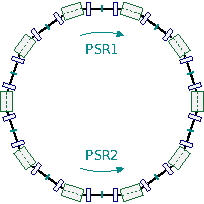
\includegraphics{Layouts/models-05}
  \caption{Ring with forward and reverse propagation.}
  \label{fig:fwd.rev.ring}
\end{marginfigure}

\index{accelerator topology!model of ring with forward and reverse propagation}
\index{ring with forward and reverse propagation!modeling}
\index{forward propagation!example}
\index{backward propagation!example}
%
Here we model an accelerator that carries a pair of
counter-propagating beams (\fref{fwd.rev.ring}, also middle
lattice in \fref{accel.models}). The two beams will propagate
through different layouts---\ptc{PRS1} for the forward-propagating
beam, and \ptc{PRS2} for the backward-propagating beam---but
the two trackable layouts must, of course, share the same ring
with the same beamline elements. They will just have different
directions of propagation and oppositely charged particles.

There is a further complication: this ring uses ``straight'' bends
instead of rectangular bends (see \fref{basic.cells}). In order to
place these elements in their proper locations, we will use the
lattice of layout \ptc{L1} as a guide, taking the ``straight''
bends from layout \ptc{L2}.%
\sidenote{The point of this complication is to illustrate some of
\PTC's geometry operations and the process of patching.
It should also, we hope, emphasize the \LEGO-block concepts of
\PTC\ (\cf\ \fref{LEGO.maps} and the associated discussion).}
The final result will be a pair of layouts, \ptc{PSR1} and
\ptc{PSR2}, each of which refer to fibres in two different
\DNA\ sequences, \ptc{L1} and \ptc{L2}.

\index{append\_empty\_layout@\ptc{append\_empty\_layout}!routine}
\index{routine!\ptc{append\_empty\_layout}}
%
We begin by calling \ptc{append_empty_layout} on \ptc{m\_u} and then
setting the layout pointer \ptc{PSR1} to point to this new layout:
%
\setptclinenums{72}{2}
\begin{ptccode}
!== PSR1 : forward ring  (layout 7)
call append_empty_layout(m_u)
PSR1 => m_u%end
\end{ptccode}
%
We shall populate this layout with a linked list of fibres taken
appropriately from layouts \ptc{L1} and \ptc{L2}. Two fibre
pointers \ptc{p1} and \ptc{p2} will step through these two layouts,
and a third fibre pointer, \ptc{f}, will keep track of our location
in \ptc{PSR1}. Elements taken from \ptc{L1} have the correct
geometric relations, but the ``straight'' bends taken from \ptc{L2}
will have to be moved to their correct locations.

\setptclinenums{76}{5}
\begin{ptccode}
p1 => L1%start
p2 => L2%start
do i = 1, L1%n
  if(p1%mag%name == "B") then
    ! read bends from L2
    call append_point(PSR1, p2)    \label{lin:psr1.append.L2}
    f => PSR1%end                  \label{lin:psr1.bgeom}
    d = p1%chart%f%o - f%chart%f%o \label{lin:psr1.comp.d}
    call translate(f, d)           \label{lin:psr1.trans.d}
    call compute_entrance_angle(f%chart%f%mid, p1%chart%f%mid, a) \label{lin:psr1.comp.a}
    call rotate(f, f%chart%f%o, a, basis = f%chart%f%mid) \label{lin:psr1.egeom}
    p2 => p2%next                  \label{lin:psr1.advance.p2}
  else
    call append_point(PSR1, p1)    \label{lin:psr1.append.L1}
  end if
  p1 => p1%next                    \label{lin:psr1.advance.p1}
end do ! elements in PSR1 now in correct locations
\end{ptccode}

\index{append\_point@\ptc{append\_point}!routine}
\index{routine!\ptc{append\_point}}
%
In the above block of code, we point \ptc{p1} and \ptc{p2}
respectively to the starts of \DNA\ sequences \ptc{L1} and \ptc{L2}.
The \ptc{do} loop over the \ptc{L1\%n} fibres in \ptc{L1} appends
to \ptc{PSR1} the desired fibres from \ptc{L1} or \ptc{L2}---bends
from \ptc{L2}, everything else from \ptc{L1}:
\begin{itemize}
  \item If \ptc{p1} points to a bend, then in \lref{psr1.append.L2}
    we append the current fibre of \ptc{L2} to \ptc{PSR1}. This, of
    course, will always be a ``straight'' bend---a \ptc{B_QUAD}.
    Later, in \lref{psr1.advance.p2}, we advance \ptc{p2} to the next
    fibre in \ptc{L2}.
  \item If \ptc{p1} does \emph{not} point to a bend, then in
    \lref{psr1.append.L1} we append the current fibre of \ptc{L1}
    to \ptc{PSR1}.
  \item In either case, we advance, in \lref{psr1.advance.p1},
    \ptc{p1} to the next fibre in \ptc{L1}.
\end{itemize}

\index{translate@\ptc{translate}!routine}
\index{routine!\ptc{translate}}
\index{compute\_entrance\_angle@\ptc{compute\_entrance\_angle}!routine}
\index{routine!\ptc{compute\_entrance\_angle}}
\index{rotate@\ptc{rotate}!routine}
\index{routine!\ptc{rotate}}
\index{global frame!used to compute local reference frame}
%
After we append a ``straight'' bend to \ptc{PSR1}, we must do
some extra work to place it in the correct location. Since we
want a given ``straight'' bend to have the same location and
orientation as the corresponding rectangular bend, we simply
compute and perform the required translations and rotations.
This happens in \lref[s]{psr1.bgeom} through \lref*{psr1.egeom}:
\label{move.elem}
\begin{enumerate}
  \item Point \ptc{f} to the fibre most recently appended to
    \ptc{PSR1}.
  \item Compute, in \lref{psr1.comp.d}, the vector \ptc{d}
    from the center of the newly appended ``straight'' bend
    (\ptc{f\%chart\%f\%o})%
    \sidenote{Read \ptc{f\%chart\%f\%o} as
    ``\ptc{f}-chart-frame-center''.}
    to the center of the corresponding
    rectangular bend in \ptc{L1} (\ptc{p1\%chart\%f\%o}).
  \item Translate the newly appended fibre (\lref{psr1.trans.d}).
  \item Compute, in \lref{psr1.comp.a}, the rotation \ptc{a}
    from the frame attached to the middle of the newly appended
    ``straight'' bend (\ptc{f\%chart\%f\%mid}) to the frame
    attached to the middle of the corresponding rectangular bend
    in \ptc{L1} (\ptc{p1\%chart\%f\%mid}).%
    \sidenote{Because rotations do not commute, their order is
    important. \PTC\ performs co\"ordinate rotations in the order
    $x$-axis, $-y$-axis, $z$-axis.}
%    Note that \ptc{a} denotes a real three-vector (see
%    \TPref{sec:init.code} \lref{decl.ad}).
  \item Rotate the newly appended fibre about its center
    (\ptc{f\%chart\%f\%o}) by angles \ptc{a}, which are given
    with respect to the frame attached to the middle of that
    element (\ptc{f\%chart\%f\%mid}).
\end{enumerate}

\index{find\_patch@\ptc{find\_patch}!routine}
\index{routine!\ptc{find\_patch}}
\index{patch!inserting}
\index{patching!find\_patch@\ptc{find\_patch} routine}
%
When the above \ptc{do} loop terminates, the beamline elements of
\ptc{PSR1} are all in their correct locations. However (recall the
discussion concerning \fref{basic.cells}) the ``straight'' bends
of \ptc{PSR1} all require patching. This happens in the following
block of code:
%
\setptclinenums{94}{5}
\begin{ptccode}
f => PSR1%start
do i = 1, PSR1%n
  if(f%mag%name == "B_QUAD") then
    call find_patch(f%previous, f, next = .true.)
    call find_patch(f, f%next, next = .false.)
  end if
  f => f%next
end do ! PSR1 now patched
\end{ptccode}
%
Within the \ptc{do} loop over all elements in \ptc{PSR1}, we apply
the patches required between each \ptc{B_QUAD} (or ``straight'' bend)
and its preceding and trailing elements. No other elements require
patching.

Finally, in the following three lines of code, we give layout \ptc{PSR1}
a formal name, and we ensure that it forms a closed topological ring,
so that particles can circulate. Note that the second two lines must
\emph{both} be executed to make the layout \ptc{PSR1} form a closed ring.
The call to \ptc{ring_L} in \lref{psr1.ringL} sets some pointers inside
the layout \ptc{PSR1} that connect the end of \ptc{PSR1} to the start,
and vice versa.
%
\setptclinenums{103}{5}
\begin{ptccode}
PSR1%name = "PSR 1"
PSR1%closed = .true.
call ring_L(PSR1, .true.) ! make it a ring topologically \label{lin:psr1.ringL}
\end{ptccode}

Query: At this point, where in the global frame are the magnets,
the ``straight'' bends, of layout \ptc{L2}?%
\sidenote{\label{sn:geom.L2}%
The geometry operations performed on the bend \ptctyp{fibre}s of
\ptc{PSR1} applied, ultimately, to the \ptctyp{element}s in \ptc{L2}.
Hence those elements are now oriented as in the right-hand layout of
\fref{DNA.subrtns}, with the global origin centered between the
adjacent ends of the top two magnets.}

To construct layout \ptc{PSR2} for the backward-propagating beam,
we follow essentially the same steps as for \ptc{PSR1}. (See the
next block of code.) There are three significant differences:
(i) In this case, all the elements are already in their proper
physical locations,${}^\text{\ref{sn:geom.L2}}$ so here we may
omit the geometric computations
and operations performed during the construction of \ptc{PSR1}.
(ii) Because of the backwards propagation, we initialize the
pointers \ptc{p1} and \ptc{p2} respectively to the \emph{ends} of
layouts \ptc{L1} and \ptc{L2}; and we advance those pointers not
to the next but to the \emph{previous} fibres in their respective
layouts. (See \lref[s]{psr2.prev2} and \lref*{psr2.prev1}.)
(iii) We must add the information that the beam described by this
layout traverses its elements in the reverse direction
(\lref{psr2.opp.dir}) and has particles with negative charge
(\lref{psr2.opp.chg}).%
\sidenote{Both direction and charge are properties of fibres,
and both default to +1.}
%
\setptclinenums{108}{5}
\begin{ptccode}
!== PSR2 : backward ring (layout 8)
call append_empty_layout(m_u)
PSR2 => m_u%end

p1 => L1%end
p2 => L2%end
do i = 1, L1%n
  if(p1%mag%name == "B") then
    call append_point(PSR2, p2)
    p2 => p2%previous            \label{lin:psr2.prev2}
  else
    call append_point(PSR2, p1)
  end if
  f => PSR2%end
  f%dir = -1                     \label{lin:psr2.opp.dir}
  f%charge = -1                  \label{lin:psr2.opp.chg}
  p1 => p1%previous              \label{lin:psr2.prev1}
end do

f => PSR2%start
do i = 1, PSR2%n
  if(f%mag%name == "B_QUAD") then
    call find_patch(f%previous, f, next = .true.)
    call find_patch(f, f%next, next = .false.)
  end if
  f => f%next
end do

PSR2%name = "PSR 2"
PSR2%closed = .true.
call ring_L(PSR2, .true.) ! make it a ring topologically
\end{ptccode}

Trackable layouts \ptc{PSR1} and \ptc{PSR2} are now complete.
Both contain 70 fibres pointing to the same set of 70 elements
in \DNA\ sequences \ptc{L1} and \ptc{L2}.


\subsection{Figure-Eight}

\index{accelerator topology!model of figure eight}
\index{figure-eight accelerator!modeling}
%
Here we model a figure-eight lattice---the left-hand lattice in
\fref{accel.models}. It carries a single beam clockwise (forward)
around the lower ring, then counter-clockwise (backward) around
the upper ring. The two rings share several elements in one
straight section. See \fref{accel.fig8}. The single trackable
layout \ptc{Fig8} we shall construct from \DNA\ sequences \ptc{L3}
and \ptc{L4} (see \tref{DNA.dbase}). For the lower ring, we use
the full ten-cell \PSR\ lattice in layout \ptc{L4}. For the upper
ring, we use all of layout \ptc{L3} (\ptc{PRS_minus}), and we
re-use six of the fibres in layout \ptc{L4}. In addition, so that
this layout does not overlap our previous layouts, \ptc{PSR1} and
\ptc{PSR2}, we shall place it \SI{40}{m} distant in the negative~$z$
direction.

\begin{figure}[ht]
  \centering
  %\includegraphics{illustrations/model-fig8}
  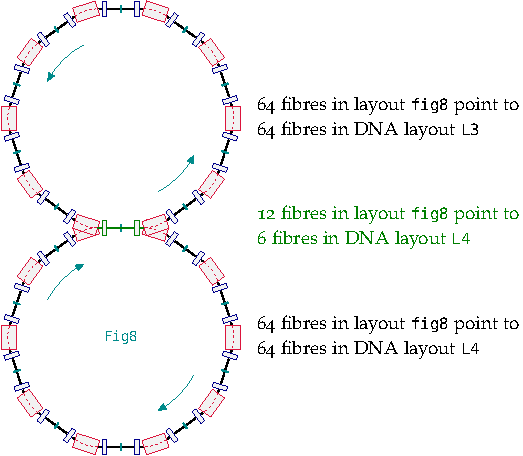
\includegraphics{Layouts/models-03}
  \caption{\ptc{Fig8} fibres pointing to elements in \ptc{L3}
           and \ptc{L4}.}
  \label{fig:accel.fig8}
\end{figure}

The construction of layout \ptc{Fig8} takes place in the following
six blocks of code. We describe each in detail.

\index{global frame!positioning first element in trackable layout}
\index{rotate@\ptc{rotate}!routine}
\index{routine!\ptc{rotate}}
%
In this first block of code, we translate layout \ptc{L4} a
distance \SI{40}{m} in the negative~$z$ direction
(\lref[s]{fig8.btr4}--\lref*{fig8.etr4}).
We then (\lref[s]{fig8.brot}--\lref*{fig8.erot}) rotate layout
\ptc{L3} \ang{180} about the entrance of its first element
(\ptc{L3\%start\%chart\%f\%a}). This rotates the gap in \ptc{L3}
down to the bottom. Now note that the bend to the right of this
gap (after the rotation) belongs to the last fibre in \ptc{L3}.
To finish placing \ptc{L3} in the correct location, we want the
\emph{end} of its last bend to coincide with the entrance of the
first bend in the lower ring, \ptc{L4}. See \fref{ring.match}.
We therefore point, in \lref{fig8.mvp1}, the fibre pointer
\ptc{p1} to the first bend (\ptc{"B"}) in \ptc{L4}; compute, in
\lref{fig8.comp.d}, the vector \ptc{d} from the exit of the last
bend in \ptc{L3} (\ptc{L3\%end\%chart\%f\%b}) to the entrance of
the first bend in \ptc{L4} (\ptc{p1\%chart\%f\%a}); and then
translate, in \lref{fig8.tr3}, layout \ptc{L3} by vector \ptc{d}.
%
\setptclinenums{141}{5}
\begin{ptccode}
!== Fig8 : figure-eight lattice (layout 9)
d = zero                                \label{lin:fig8.btr4}
d(3) = -40.d0
call translate(L4, d)                   \label{lin:fig8.etr4}
a = zero                                \label{lin:fig8.brot}
a(2) = pi
call rotate(L3, L3%start%chart%f%a, a)  \label{lin:fig8.erot}
call move_to(L4, p1, "B", pos)          \label{lin:fig8.mvp1}
d = p1%chart%f%a - L3%end%chart%f%b     \label{lin:fig8.comp.d}
call translate(L3, d)                   \label{lin:fig8.tr3}
\end{ptccode}
%
At this point, the beamline elements for the figure-eight lattice
are all correctly located and oriented.

\begin{marginfigure}[-29\baselineskip]\forceversofloat
  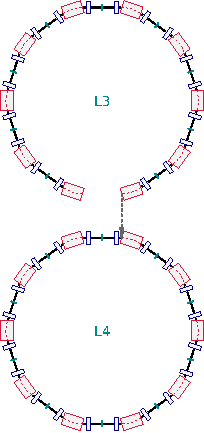
\includegraphics{Layouts/models-06}
  \caption{Matching \ptc{L3} to \ptc{L4}.}
  \label{fig:ring.match}
\end{marginfigure}

\index{append\_empty\_layout@\ptc{append\_empty\_layout}!routine}
\index{routine!\ptc{append\_empty\_layout}}
%
In the next block of code, we first call \ptc{append_empty_layout}
on \ptc{m_u} and set the layout pointer \ptc{Fig8} to point to this
new layout. Then, in \lref[s]{fig8.bapp.L4}--\lref*{fig8.eapp.L4},
we append in order all the fibres of \ptc{L4} to \ptc{Fig8}.
%
\setptclinenums{152}{5}
\begin{ptccode}
call append_empty_layout(m_u)
Fig8 => m_u%end
p1 => L4%start                 \label{lin:fig8.bapp.L4}
do i = 1, L4%n
  call append_point(Fig8, p1)
  p1 => p1%next                \label{lin:fig8.p1next}
end do                         \label{lin:fig8.eapp.L4}
\end{ptccode}
%
We now have the complete lower ring.

\index{append\_point@\ptc{append\_point}!routine}
\index{routine!\ptc{append\_point}}
\index{doko!described}
%
In the next block of code, we start to include the upper ring by
appending to \ptc{Fig8} the first three fibres of the lower ring.
These three new fibres in \ptc{Fig8} will, of course, point to the
same physical elements as do the first three fibres in \ptc{Fig8}:
a long drift, a defocusing quadrupole, and a short drift. During
the calls to \ptc{append_point}, \PTC\ will add this information
to the \ptc{doko}s of the corresponding elements in \ptc{L4}. As a
consequence, each of those three elements in \DNA\ sequence \ptc{L4}
knows that it is pointed to by two different fibres in trackable
layout \ptc{Fig8}.%
\sidenote{Each of those elements already knows it belongs to a
fibre in layout \ptc{L4}.}

Note that we need not initialize the pointer \ptc{p1} to \ptc{L4\%start}: the last execution, in \lref{fig8.p1next}, of \ptc{p1 => p1\%next} returns \ptc{p1} to the beginning of the layout.
%
\setptclinenums{160}{5}
\begin{ptccode}
write(6,*) p1%mag%name
call append_point(Fig8, p1)
p1 => p1%next
write(6,*) p1%mag%name
call append_point(Fig8, p1)
p1 => p1%next
write(6,*) p1%mag%name
call append_point(Fig8, p1)
\end{ptccode}

In the next block of code, we append the fibres of layout \ptc{L3}
to \ptc{Fig8}. Since our beam traverses \ptc{L3} in the reverse
direction, we initialize the fibre pointer \ptc{p1} to \ptc{L3\%end}
(\lref{fig8.p1.set1}), and we advance that pointer to the
\emph{previous} fibre (\lref{fig8.prev1}). During this process,
we take care of two other tasks: We tell \PTC\ that these elements
are traversed in the reverse direction (\lref{fig8.opp.dir}); and,
if the element is a bend, we reverse the sign of the magnetic field
(\lref{fig8.revb}). The particle charge remains the same (default
value +1).
%
\setptclinenums{169}{5}
\begin{ptccode}
p1 => L3%end                   \label{lin:fig8.p1.set1}
do i = 1, L3%n
  call append_point(Fig8, p1)
  Fig8%end%dir = -1            \label{lin:fig8.opp.dir}
  if(p1%mag%name == "B") p1%mag%bn(1) = -p1%mag%bn(1) \label{lin:fig8.revb}
  p1 => p1%previous            \label{lin:fig8.prev1}
end do
\end{ptccode}

\index{doko!described}
%
To complete the upper ring, and hence our trackable layout
\ptc{Fig8}, three fibres remain to be appended: the last three
fibres of the lower ring, \ptc{L4}. This is accomplished in the
next block of code. First, in \lref{fig8.p1.set2}, we point
\ptc{p1} to the fibre containing the short drift near the end of
layout \ptc{L4}. We then append to \ptc{Fig8} that fibre and the
next two. During the calls to \ptc{append_point}, \PTC\ will add
the appropriate information to the \ptc{doko}s of the corresponding
elements.
%
\setptclinenums{177}{5}
\begin{ptccode}
p1 => L4%end%previous%previous  \label{lin:fig8.p1.set2}
write(6,*) p1%mag%name
call append_point(Fig8, p1)
p1 => p1%next
write(6,*) p1%mag%name
call append_point(Fig8, p1)
p1 => p1%next
write(6,*) p1%mag%name
call append_point(Fig8, p1)
\end{ptccode}

\index{check\_need\_patch@\ptc{check\_need\_patch}!routine}
\index{routine!\ptc{check\_need\_patch}}
\index{find\_patch@\ptc{find\_patch}!routine}
\index{routine!\ptc{find\_patch}}
\index{patch!inserting}
\index{patch!checking whether needed}
\index{patching!\ptc{find\_patch} routine}
\index{patching!\ptc{check\_need\_patch} routine}
%
Finally, in the last block of code for \ptc{Fig8}, we give our new
layout a formal name (\ptc{"Figure-Eight"}), ensure that it is
topologically closed, and apply any necessary patches. The call to
\ptc{check_need_patch}, \lref{fig8.chk.patch}, returns the integer
\ptc{pos} equal to zero if no patch is needed. A non-zero value
indicates the type of patch required. By using \ptc{check_need_patch},
we can apply patches only where necessary. Our figure-eight lattice
requires patching because some of the constituent elements are
traversed in the reverse direction. In particular, there are adjacent
fibres \ptc{f} which have opposite values of \ptc{f\%dir}. This
happens between the short drift at end of the common straight section
and the first bend of the upper ring; and also between the last bend
of the upper ring and the subsequent short drift.
%
\setptclinenums{187}{5}
\begin{ptccode}
write(6,*) "Fig8 has ", Fig8%n, " fibres"
Fig8%name = "Figure-Eight"
Fig8%closed = .true.
call ring_L(Fig8, .true.) ! make it topologically closed

p1 => Fig8%start
do i = 1, Fig8%n
  call check_need_patch(p1, p1%next, 1.d-10, pos)  \label{lin:fig8.chk.patch}
  if(pos /= 0) call find_patch(p1, p1%next, next = .false.)
  p1 => p1%next
end do
\end{ptccode}

Trackable layout \ptc{Fig8} is now complete. It has 140~fibres
pointing to 134~elements in \DNA\ sequences \ptc{L4} and \ptc{L3}.
Twelve of the fibres in \ptc{Fig8} point to the six elements (four
drifts and two quadrupoles at the top of \ptc{L4}) which are common
to the upper and lower rings. See \fref{accel.fig8}.


\subsection{Collider}

\begin{marginfigure}
  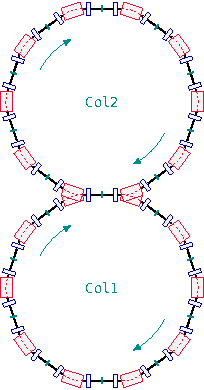
\includegraphics{Layouts/models-07}
  \caption{Collider.}
  \label{fig:col1.col2}
\end{marginfigure}

\index{accelerator topology!model of collider}
\index{collider!modeling}
%
Here we model a collider---\fref{col1.col2}, also the right-hand
lattice in \fref{accel.models}---which has clockwise propagating
beams in each of its two rings. This model comprises two layouts,
\ptc{Col1} and \ptc{Col2}, which we shall construct from
\DNA\ sequences \ptc{L5} and \ptc{L6} (see \tref{DNA.dbase}). For
the lower ring, we use the full ten-cell \PSR\ lattice in layout
\ptc{L6}. For the upper ring, we use all of layout \ptc{L5}
(\ptc{PRS_minus}), and we re-use six of the fibres in layout
\ptc{L6}.%
\sidenote{Yes, this sounds much like the description for layout
\ptc{Fig8}. Be sure to note the \emph{differences}.}
In addition, so that this layout does not overlap our previous
layouts, \ptc{PSR1}, \ptc{PSR2}, and \ptc{Fig8}, we shall place
it \SI{40}{m} distant in the positive~$z$ direction.

The construction of layouts \ptc{Col1} and \ptc{Col2} takes place
in the following four blocks of code. We describe each in detail.

In this first block of code, we place all the beamline elements of
layouts \ptc{Col1} and \ptc{Col2} in their correct locations: We
translate layout \ptc{L6} a distance \SI{40}{m} in the positive~$z$
direction. We then rotate layout \ptc{L5} \ang{180} about the
entrance of its first element (\ptc{L5\%start\%chart\%f\%a}). This
rotates the gap in \ptc{L5} down to the bottom. To finish placing
\ptc{L5} in the correct location, we want the \emph{end} of its
last bend to coincide with the entrance of the first bend in the
lower ring, \ptc{L6}. We therefore point layout pointer \ptc{p1}
to the first bend (\ptc{"B"}) in \ptc{L6}; compute the vector
\ptc{d} from the exit of the last bend in \ptc{L5}
(\ptc{L5\%end\%chart\%f\%b}) to the entrance of the first bend in
\ptc{L6} (\ptc{p1\%chart\%f\%a}); and then translate layout \ptc{L5}
by that vector \ptc{d}.
%
\setptclinenums{200}{5}
\begin{ptccode}
!== Col1 : lower collider ring (layout 10)
!== Col2 : upper collider ring (layout 11)
d = zero
d(3) = 40.d0
call translate(L6, d)
a = zero
a(2) = pi
call rotate(L5, L5%start%chart%f%a, a)
call move_to(L6, p1, "B", pos)
d = p1%chart%f%a - L5%end%chart%f%b
call translate(L5, d)
\end{ptccode}

\index{append\_empty\_layout@\ptc{append\_empty\_layout}!routine}
\index{routine!\ptc{append\_empty\_layout}}
\index{append\_point@\ptc{append\_point}!routine}
\index{routine!\ptc{append\_point}}
%
In the next block of code, we construct layout \ptc{Col1}: We
call \ptc{append_empty_layout} on \ptc{m_u} and set the layout
pointer \ptc{Col1} to point to this new layout. Then we append
in order all the fibres of \ptc{L6} to \ptc{Col1}. Finally, we
give our new layout a formal name (\ptc{"Collider 1"}) and ensure
that it is topologically closed. This layout does not require
patching.
%
\setptclinenums{212}{5}
\begin{ptccode}
call append_empty_layout(m_u)
Col1 => m_u%end
p1 => L6%start
do i = 1, L6%n
  call append_point(Col1, p1)
  p1 => p1%next
end do

write(6,*) "Collider 1 has ", Col1%n, " fibres"
Col1%name = "Collider 1"
Col1%closed = .true.
call ring_L(Col1, .true.) ! make it a ring topologically
\end{ptccode}

In the next block of code, we construct layout \ptc{Col2}: We call
\ptc{append_empty_layout} again on \ptc{m_u}, set the layout
pointer \ptc{Col2} to point to this new layout, and then locate,
in \lref{col2.next.next}, the first short drift in layout \ptc{L6}.
To populate \ptc{Col2}, we now, in
\lref[s]{col2.bapp.str}--\lref*{col2.eapp.str}, march backwards
appending the six elements in the straight section at the top of
layout \ptc{L6} (short drift, defocusing quadrupole, two long drifts,
focusing quadrupole, and short drift). While doing this, we inform
\PTC, in \lref{col2.opp.dir}, that this layout traverses those
elements in the opposite direction. Finally, in
\lref[s]{col2.bapp.L5}--\lref*{col2.eapp.L5}, we append in order all
the fibres of \ptc{L5} to \ptc{Col2}.
%
\setptclinenums{225}{5}
\begin{ptccode}
call append_empty_layout(m_u)
Col2 => m_u%end
p1 => L6%start%next%next    \label{lin:col2.next.next}
do i = 1, 6                 \label{lin:col2.bapp.str}
  write(6,*) p1%mag%name
  call append_point(Col2, p1)
  Col2%end%dir = -1         \label{lin:col2.opp.dir}
  p1 => p1%previous
end do                      \label{lin:col2.eapp.str}
p1 => L5%start              \label{lin:col2.bapp.L5}
do i = 1, L5%n
  call append_point(Col2, p1)
  p1 => p1%next
end do                      \label{lin:col2.eapp.L5}
\end{ptccode}

\index{check\_need\_patch@\ptc{check\_need\_patch}!routine}
\index{routine!\ptc{check\_need\_patch}}
\index{find\_patch@\ptc{find\_patch}!routine}
\index{routine!\ptc{find\_patch}}
\index{patch!inserting}
\index{patch!checking whether needed}
\index{patching!\ptc{find\_patch} routine}
\index{patching!\ptc{check\_need\_patch} routine}
%
In this last block of code for \ptc{Col2}, we give our new layout a
formal name (\ptc{"Collider 2"}), ensure that it is topologically
closed, and apply any necessary patches. This layout requires patches
only where \ptctyp{fibre}\ptc{\%dir} switches sign. As in our earlier
layout \ptc{Fig8}, this happens at the two ends of the common straight
section, where they join the bends of the upper ring.
%
\setptclinenums{240}{5}
\begin{ptccode}
write(6,*) "Collider 2 has ", Col2%n, " fibres"
Col2%name = "Collider 2"
Col2%closed = .true.
call ring_L(Col2, .true.) ! make it a ring topologically

p1 => Col2%start
do i = 1, Col2%n
  call check_need_patch(p1, p1%next, 1.d-10, pos)
  if(pos /= 0) call find_patch(p1, p1%next, next = .false.)
  p1 => p1%next
end do
\end{ptccode}

The trackable layouts \ptc{Col1} and \ptc{Col2} are now complete.
They have 140 fibres pointing to 134 elements in \DNA\ sequences
\ptc{L6} and \ptc{L5}. Twelve of the fibres in \ptc{Col1} and
\ptc{Col2} point to the six elements which are common to the upper
and lower rings.


\section{DNA Arrays}
\label{sec:DNA.array}

\index{DNA array!described}
\index{layout!trackable}
\index{DNA database!storing trackable layouts}
\index{allocate@\ptc{allocate}!routine}
\index{routine!\ptc{allocate}}
%
The following code constitutes a bit of housekeeping. We have created a set of six layouts---\ptc{L1}--\ptc{L6}---that form the core of our \DNA\ database. What we do here is tell each of the trackable layouts we have created---\ptc{PSR1}, \ptc{PSR2}, \ptc{Fig8}, \ptc{Col1}, and \ptc{Col2}---which \DNA\ sequences they use. This information is stored in the array \ptc{DNA} that is part of the data held in each \PTC\ \ptctyp{layout}.

In \lref{dna.L1} we record in \ptc{PSR1} the fact that \DNA\ sequence \ptc{L1} is used by \ptc{PSR1}. Then \lref{dna.L2} records the fact that \ptc{PSR1} also uses \DNA\ sequence \ptc{L2}. Note that this latter line makes use of the linked-list character of our \DNA\ database. (Recall, see \pref{mad.univ}, that \ptc{m_u} is a linked list of layouts.) Since \ptc{PSR1\%DNA(1)\%L} already points to \ptc{L1} (see \lref{dna.L1}), and since \ptc{L2} is the next layout in the \DNA\ database, then \ptc{PSR1\%DNA(1)\%L\%next} points to \ptc{L2}. (In this very simple case you could, of course, replace \lref[s]{dna.bdo}--\lref*{dna.edo} with the single statement \ptc{PSR1\%DNA(2)\%L => L2}.) The remaining lines in this block of code populate the \DNA\ arrays for the other trackable layouts.
%
\setptclinenums{257}{5}
\begin{ptccode}
allocate(PSR1%DNA(2))
PSR1%DNA(1)%L => L1                           \label{lin:dna.L1}
do i = 2, 2                                   \label{lin:dna.bdo}
  PSR1%DNA(i)%L => PSR1%DNA(i-1)%L%next ! L2  \label{lin:dna.L2}
end do                                        \label{lin:dna.edo}

allocate(PSR2%DNA(2))
PSR2%DNA(1)%L => L1
do i = 2, 2
  PSR2%DNA(i)%L => PSR2%DNA(i-1)%L%next ! L2
end do

allocate(Fig8%DNA(2))
Fig8%DNA(1)%L => L3
do i = 2, 2
  Fig8%DNA(i)%L => Fig8%DNA(i-1)%L%next ! L4
end do

allocate(Col1%DNA(2))
Col1%DNA(1)%L => L5
do i = 2, 2
  Col1%DNA(i)%L => Col1%DNA(i-1)%L%next ! L6
end do

allocate(Col2%DNA(2))
Col2%DNA(1)%L => L5
do i = 2, 2
  Col2%DNA(i)%L => Col2%DNA(i-1)%L%next ! L6
end do
\end{ptccode}


\makeussubscript
\endinput
